% file siminos/froehlich/slice/slice.tex
% $Author$ $Date$

% \section{Dynamics in the slice}
% \section{\Mslices} % OLD
%       \label{sec:mslices}



Any \statesp\ trajectory can be written in a factorized
form $\ssp(\tau)=\LieEl(\tau)
\sspRed(\tau)$. Differentiating both sides with respect to time and
setting $\velRed={d\sspRed}/{d\tau}$ we find
\(
\vel(\ssp)=\dot{\LieEl} \, \sspRed+\LieEl \, \velRed(\sspRed)
\,.
\)
By the equivariance \refeq{eq:FiniteRot}
\[
\vel=\velRed + \LieEl^{-1} \, \dot{\LieEl} \, \sspRed
\,.
\]
The product $\LieEl^{-1}\dot{\LieEl}$ defines
the group tangent:
$\LieEl^{-1}\dot{\LieEl}=e^{-\gSpace \cdot \Lg} \,
\frac{d ~~}{d \, \tau} e^{\gSpace \cdot \Lg}=\dot{\gSpace}\cdot \Lg$,
leaving us with the equation for the velocity of the reduced flow in the slice:
\beq
\velRed(\sspRed)=\vel(\sspRed)-\dot{\gSpace}(\sspRed)\cdot \groupTan(\sspRed).
\ee{eq:redVel}
In other words, the velocity in the full \statesp\ is the sum of the
velocity normal along the group tangent and the remainder $\velRed$.

This equation is true for any factorization $\ssp(\tau)=\LieEl(\tau)
\sspRed(\tau)$, and by itself provides no information on how to calculate
$\dot{\gSpace}$. Let
$\sliceTan{a}$ be the group tangents at the slice
fixing point. Requirement that the flow is confined to the slice,
as in \refeq{PCsectQ0},
we find that $\dot{\gSpace}$ must satisfy
\beq
\braket{\vel(\sspRed)}{\sliceTan{a}}
 -\braket{\dot{\gSpace}\cdot \groupTan(\sspRed)}{\sliceTan{a}}=0
\,.
\label{eq:slicecondition}
\eeq
% for each group tangent $\sliceTan{a}$ at the slice fixing point.
In principle\rf{FiSaScWu96} this is a matrix equation one can solve
for $\dot{\gSpace}_a$. Here we shall consider only the easiest case,
$\SOn{2}$ which has a single group tangent:
\bea
\velRed(\sspRed) &=& \vel(\sspRed)
   -\dot{\gSpace}(\sspRed) \groupTan(\sspRed)
\continue
\dot{\gSpace}(\sspRed) &=& \frac{\braket{\vel(\sspRed)}{\sliceTan{}}}
               {\braket{\groupTan(\sspRed)}{\sliceTan{}}}
\,.
\label{eq:so2reduced}
\eea
The first equation defines the flow confined to the slice, and
integration of the second, `reconstruction'
equation\rf{Marsd92,cont:MarsdRat94} enables us to reconstruct the
corresponding trajectory in the full \statesp.
 \begin{figure}
 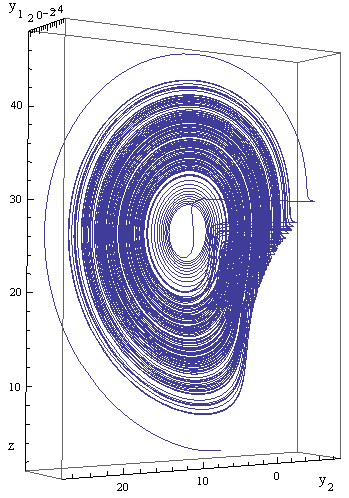
\includegraphics[width=0.35\textwidth]{CLEreduced}%
 \caption{\label{fig:CLErx2y1z}
A $\{y_1,y_2,z\}$ plot of the \reducedsp\ \cLf\ strange attractor
with initial point
%$(x_1, x_2, y_1, y_2, z) = (1, 2, 3, 1, 2)$
in the
slice normal to $\sliceTan{}=(1,0,0,0,0)$. Contrast this plot with
\reffig{fig:CLEx2y1z}, and note the apparent discontinuities in the
reduced flow.
 }%
 \end{figure}

%\item[2010-12-06 PC]
%\HREF{http://webusers.physics.uiuc.edu/~goldbart/PostScript/MS_PG_book/bookmaster.pdf}
{Stone and Goldbart}\rf{StGo09} Sect 1.5 discussion of Lagrange
multipliers, simple and intuitive, suggests that we should think of
symmetry reduction of dynamics to a slice in terms of Lagrange
multipliers. Perhaps we can finally get a clear exposition that unifies
our discussion of \Poincare\ sections and \reducedsp\ with our methods of
finding \po s and \rpo s, where we increase dimension by one for every
continuous symmetry dimension. Rytis starting writing that up for
ChaosBook (it is in the boyscout edition) but characteristically left in
limbo.



%
% ****** End of file slice.tex ******
